\documentclass[letter, 10pt]{article}
\usepackage[utf8]{inputenc}
\usepackage[spanish]{babel}
\usepackage{amsfonts}
\usepackage{amsmath}
\usepackage{subfig}
\usepackage{graphicx}
\graphicspath{ {images/} }
\usepackage{url}
\usepackage[top=3cm,bottom=3cm,left=3.5cm,right=3.5cm,footskip=1.5cm,headheight=1.5cm,headsep=.5cm,textheight=3cm]{geometry}


\begin{document}
\title{Inteligencia Artificial \\ \begin{Large}Estado del Arte: Progressive Party Problem\end{Large}}
\author{[Roberto Fuentes Zenteno]}
\date{\today}
\maketitle


%--------------------No borrar esta secci\'on--------------------------------%
\section*{Evaluaci\'on}

\begin{tabular}{ll}
Resumen (5\%): & \underline{\hspace{2cm}} \\
Introducci\'on (5\%):  & \underline{\hspace{2cm}} \\
Definici\'on del Problema (10\%):  & \underline{\hspace{2cm}} \\
Estado del Arte (35\%):  & \underline{\hspace{2cm}} \\
Modelo Matem\'atico (20\%): &  \underline{\hspace{2cm}}\\
Conclusiones (20\%): &  \underline{\hspace{2cm}}\\
Bibliograf\'ia (5\%): & \underline{\hspace{2cm}}\\
 &  \\
\textbf{Nota Final (100\%)}:   & \underline{\hspace{2cm}}
\end{tabular}
%---------------------------------------------------------------------------%
\vspace{2cm}


\begin{abstract}
Se presenta el problema \textit{Progressive Party Problem} (PPP), propuesto por Peter Hubbard (\textit{Southampton
University}). Consiste en organizar de la mejor manera una ``fiesta progresiva'' en un grupo de yates, en donde durante periodos consecutivos de tiempo la tripulación de los yates invitados debe visitar los yates anfitriones. El objetivo del problema es asignar todas las tripulaciones visitantes a los yates anfitriones para cada período de tiempo, minimizando la cantidad de yates anfitriones. Se describe el problema, luego se analiza el estado actual del problema mediante el estado del arte, seguido de un modelo matemático, además de las técnicas que se han usado para abordarlo y los resultados acotados que se han obtenido. 
\textbf{Keywords}: PPP, optimización combinatoria, programación lineal entera, programación de restricciones,busqueda local.
\end{abstract}

\section{Introducción}
Una conferencia es una manera excelente en que las personas que tienen intereses comunes pueden reunirse e intercambiar las ideas m\'as vanguardistas de su campo. Es por esto que la gestión de eventos progresivos es un elemento importante a controlar y mejorar. En este documento, se presenta el \textit{Progressive Party Problem} (PPP), problema especifico que plante\'o Peter Hubbard, miembro de la asociación \textit{Sea Wych Owners} y del departamento de matematicas de \textit{Southampton University} en el a\~no 1996~\cite{Kalvelagen20031713}, cuyo objetivo es asignar todas las tripulaciones visitantes a los yates anfitriones para cada período de tiempo, minimizando la cantidad de yates anfitriones. El documento proporciona el planteamiento del problema bien definido junto con su formulación a través de Programación entera y Programación de restricciones junto a una explicación de como fueron los resultados de ambos experimentos. Además, existen otros documentos donde se entrega la data del problema y sus respectivas soluciones usando distintas técnicas, junto a los tiempos que demoraron y las máquinas donde se testearon.
\\

\textit{Progressive Party Problem} (PPP) busca encontrar la mejor manera de gestionar yates invitados y anfitriones, donde los yates invitados podrán invitar a los anfitriones en determinados periodos de tiempo. Su objetivo es minimizar los yates anfitriones respetando ciertas restricciones, como evitar exceder la cantidad de los yates anfitriones o que las tripulaciones invitadas no podrán toparse más de una vez.
\\

La motivación del problema surge debido al problema originado en \textit{Bembridge}, Isla de \textit{Wight}~\cite{Kalvelagen20031713}. Su contexto es organizar un programa social para un paseo de yates, donde estos estaban amarrados en un puerto deportivo. Para que las personas se reúnan con tantos otros asistentes como les fuera posible, se planeó una fiesta nocturna en donde algunos de estos yates serian designados como anfitriones, y las tripulaciones de los barcos restantes irían visitando a estos yates anfitriones durante seis horas en periodos de media hora. El problema que enfrentaba el organizador del paseo era el de minimizar el número de los barcos anfitriones, ya que cada anfitrión tenía que ser abastecido con alimentos y otros prerrequisitos. 

La estructura del actual trabajo es la siguiente: En la sección siguiente se define y se explica detalladamente el problema \textit{Progressive Party Problem}, en la sección 3 se plantea el estado del arte del problema analizado, indicando los soluciones encontradas hasta el día de hoy. Luego en la sección 4 se presenta el modelo matemático que mejor resuelve el problema con el fin de que cualquier persona sea capaz de interpretarlo. Finalmente en la sección 5 se concluye sobre el problema estudiado.

\section{Definición del Problema}
\subsection{Progressive Party Problem}
\subsubsection{Definición}
\textit{Progressive Party Problem} (PPP) busca encontrar la mejor manera de gestionar yates invitados y anfitriones, donde los yates invitados podrán invitar a los anfitriones en determinados periodos de tiempo. 

\subsubsection{Objetivo}
El objetivo de PPP es asignar todas las tripulaciones visitantes a los yates anfitriones para cada período de tiempo, minimizando la cantidad de yates anfitriones.

\subsubsection{Parametros}
\textit{Progressive Party Problem} tiene los siguientes parámetros:

\begin{itemize}
\item $H$: Cantidad de yates.
\item $K_i$: Capacidad del yate $i$.
\item $T$: cantidad de períodos.
\item $c_i$: cantidad de tripulantes del yate $i$.
\item $H_i$: 1 si el yate $i$ es un anfitrión.
\item $G_{ikt}$: 1 si el yate $k$ es un invitado del yate $i$ en el período $t$
\item $m_{klt}$:  1 si el yate $k$ y $l$ se encuentran en el período $t$.
\end{itemize}

\subsubsection{Variables}
Algunas variables de PPP son las siguientes:

    \begin{itemize}
      \item $h_i$: 1 si el yate $i$ es un yate anfitrión.
      \item $x_{ikt}$: 1 si el yate $k$ es un invitado del bote $i$ en el periodo $t$.
    \end{itemize}

\subsubsection{Restricciones}
\begin{itemize}
\item Un yate solo podrá ser visitado si es un yate anfitrión.
\item La capacidad de los yates anfitriones no se puede exceder.
\item Cada tripulación debe siempre tener un anfitrión asociado o ser uno.
\item Una tripulación invitada no podrá visitar un yate anfitrión más de una vez.
\item Las tripulaciones invitadas no podrán toparse más de una vez.
\end{itemize}

\subsection{Otras variantes}
Tenemos varios problemas relacionados con la gestión de yates, los cuales buscan distintas maneras de resolver el problema: Como un CSP, maximizar la duración de la fiesta, definir diferentes restricciones del problema. Las variantes clásicas son:

\begin{enumerate}
    \item \textbf{PPP as CSP}: \\
    Ver si es factible o no realizar una fiesta con las características dadas. Lo que se busca es encontrar una instanciación de las variables que cumpla con las restricciones descritas del problema (y sin una función objetivo). ~\cite{Brailsford:1996:OSE:241748.241755}
    
     \item \textbf{Uncapacited CPP}:\\
     Otra de las variantes del \textit{Progressive Party Problem} es resolver el problema sin considerar la capacidad de los barcos. Si ignoramos las restricciones de capacidad, sólo un barco anfitrión puede acomodar cualquier número de barcos invitados por un período de tiempo. Durante más de un período de tiempo, podemos encontrar fácilmente un límite inferior en el número de anfitriones requeridos del argumento siguiente. Por lo anterior, para el caso particular de 42 botes en total, 7 serán anfitriones y 35 invitados.
     
     Si $g$ tripulaciones visitan al $host$ $i$ en el periodo 1, entonces debe haber por lo menos $g$ otros anfitriones para poder distribuirlos a todos en el siguiente período de tiempo (Los huéspedes no pueden visitar un anfitrión $i$ otra vez, y deben visitar los $g$ anfitriones  diferentes para no reunirse con otra tripulación nuevamente). De hecho, los $g + 1$ anfitriones requeridos podrían acomodar a las $g$ tripulaciones en el periodo 1 sin que estos se encuentren nuevamente en el periodo 2, dando $g(g + 1)$ invitados en total.
Por más de 2 períodos de tiempo, $g (g + 1)$ es claramente un límite superior en el número de invitados que g + 1 $hosts$ pueden acomodar. De hecho, estos límites pueden ser alcanzados (aún suponiendo que no hay limitaciones en las capacidades de los anfitriones, y siempre que el número de períodos de tiempo no sea mayor que el número de anfitriones, en cuyo caso se hace imposible que las tripulaciones de invitados no visiten el mismo anfitrión más de una vez).

     El problema recae en la vida real, donde los yates poseen una capacidad máxima, por lo que este enfoque no es el mas indicado para resolver el problema, Además de que el numero necesario de anfitriones para esta variante es de mínimo 13 anfitriones. ~\cite{Smith1996}

    \item \textbf{A Lower Bound}: \\ 
    Un límite inferior en el número de yates anfitriones necesarios (teniendo en cuenta las limitaciones de capacidad) se encontró mediante la programación lineal para relajar de forma considerable el problema. Esto simplemente requería que las tripulaciones invitadas tuvieran en cuenta la capacidad de reserva total de los barcos anfitriones durante un período de tiempo. Este límite se puede encontrar alternativamente a partir de un simple argumento: una condición necesaria para la viabilidad es que la capacidad total de los barcos de acogida sea mayor que el tamaño total de la tripulación de todos los barcos, por lo que el menor número de huéspedes que cumplen con esta condición se encuentra ordenando los barcos en orden descendente de capacidad total. Con esto, los primeros 13 barcos pueden acomodar a todas las tripulaciones; Los primeros 12 barcos no pueden. Esto sugiere que en general los barcos anfitriones deben ser elegidos en orden descendente de capacidad total (Se toma como una heurística).~\cite{Smith1996}

\end{enumerate}

\section{Estado del Arte}
Hoy en día los eventos o conferencias son excelentes maneras en que personas con intereses en común puedan reunirse e intercambiar ideas. Para poder gestionar de mejor manera estos eventos, podemos trabajar estos casos como problemas de planificación de tiempo (\textit{Scheduling Problem}), donde un caso particular es el \textit{Progressive Party Problem} (PPP). 

\begin{figure}[ht!]
 \centering
  \subfloat[Fiesta de yates, \textit{Island of Wight}]{
   \label{f:Fiesta yates}
    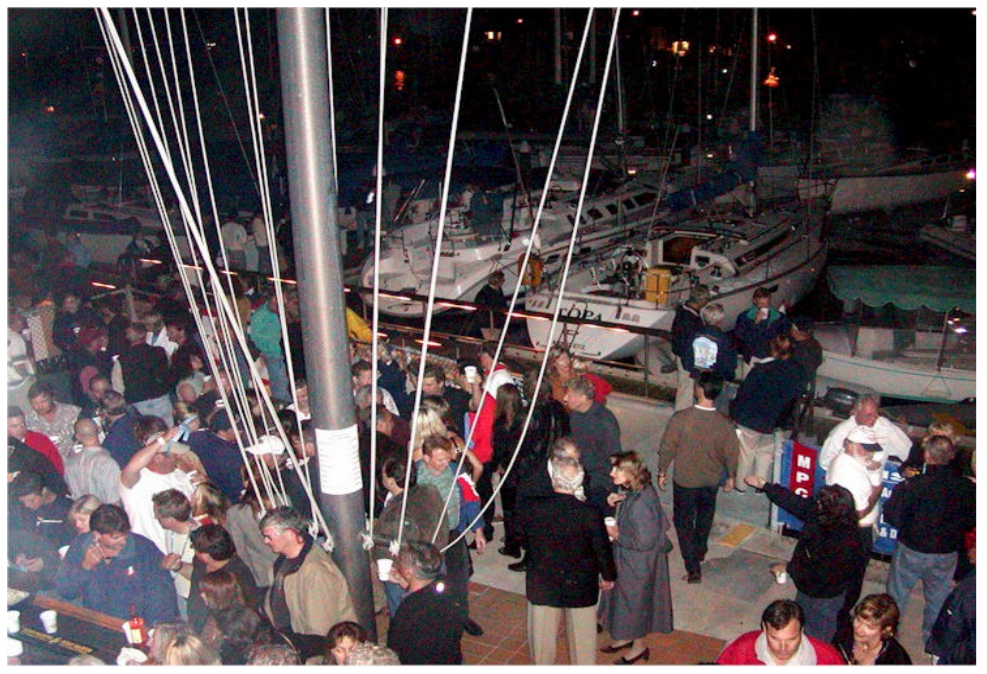
\includegraphics[width=0.5\textwidth]{party1.png}}
  \subfloat[Vista general de PPP]{
   \label{f:Vista general}
    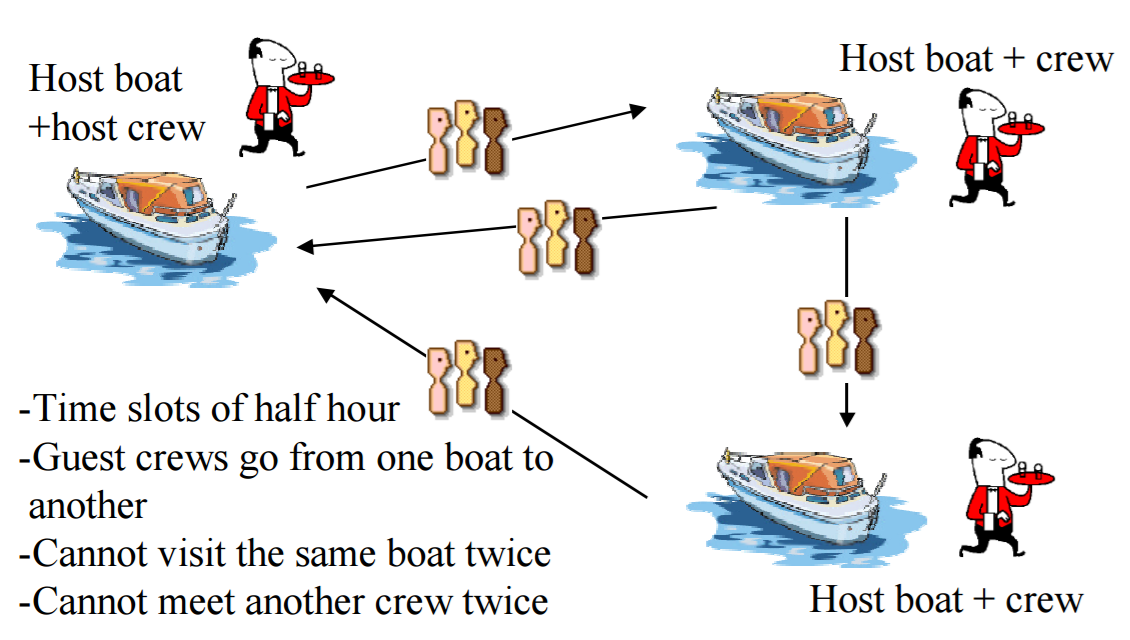
\includegraphics[width=0.5\textwidth]{party2.png}}
 \caption{Progressive Party Problem}
 \label{f:PPP}
\end{figure}

El problema fue originalmente propuesto por Peter Hubband de la Universidad de \textit{Southampton}, organizador de un club de yates con 42 botes y sus tripulaciones respectivas. Este importante evento nocturno tiene como objetivo organizar una fiesta donde cada tripulación socializa con tantas otras tripulaciones como le sea posible. El problema ahora es asignar todos los equipos invitados a los barcos anfitriones para cada uno de los intervalos de tiempo, utilizando el número mínimo de barcos anfitriones. Con el paso del tiempo, se van planteando más problemas con distintos objetivos referidos a la planificación de eventos, lo que da origen a todas las variantes que se mencionaron anteriormente. Es importante destacar que los primeros 3 yates serán yates anfitriones puesto que el primer yate es del organizador del evento, y los 2 siguientes contienen tripulaciones con niños. Las tripulaciones se separaron para que los padres permanecieran a bordo del
barco anfitrión, por lo que los niños se convirtieron en un \textbf{"barco virtual"} con capacidad cero. En conjunto con los niños del yate del organizador del evento se formaron tres barcos virtuales, sumando un total de 42 botes:

\begin{figure}[ht]
\centering
 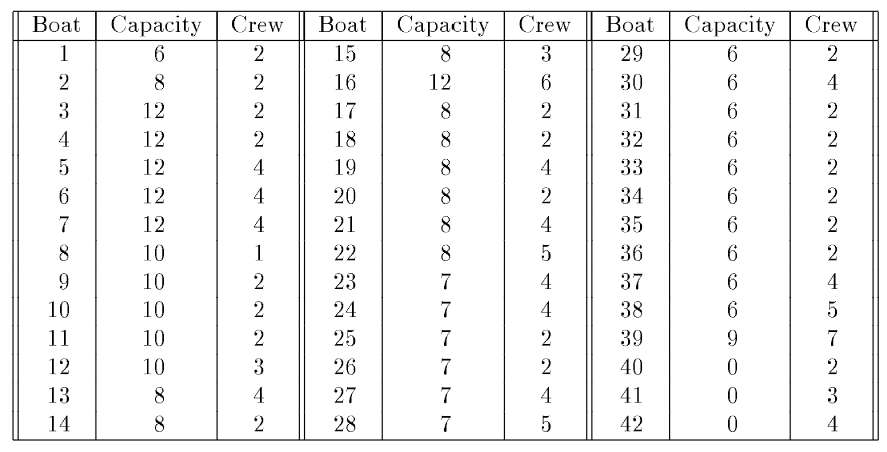
\includegraphics[width=0.8\textwidth]{party5.png}
 \caption{Data del problema real}
\end{figure}

En el paper \textit{The progressive party problem: Integer linear programming and constraint programming compared} ~\cite{Smith1996} se proponen dos tipos de modelos: a través de ILP (\textit{Integer-Linear Programming} ) y CP (\textit{Constraint Programming}). El documento nos habla de que a pesar de que ILP pareciera ser el método mas poderoso para resolver nuestro problema, a veces la programación de restricciones puede resolver estos problemas mas rápido. La formulación con programación lineal entera incluyendo todas las restricciones recae en un modelo muy largo. Probando varias estrategias nos damos cuenta de que lamentablemente todos los intentos de solución fallan. Por otra parte la programación de restricciones puede resolver este problema rápidamente, con un poco de ayuda manual. 

\begin{itemize}
\item \textbf{Enfoque con programación entera}
\begin{itemize}    
\item 
Luego de proponer el modelo con programación entera, se determinó que el numero de filas (restricciones) es de $O(B^4T^2)$, siendo $B$ el numero de barcos y $T$ el numero de periodos, y el numero de variables es de $O(B^2T)$. Aquí el problema es reducido puesto que se considera que en cualquier solución óptima se encuentran yates que siempre sera escogidos para ser anfitriones debido a su gran capacidad y pequeño tamaño de tripulantes. Por esto mismo algunos barcos jamas serán escogidos como barcos anfitriones (por ejemplo los barcos virtuales con capacidad 0). Los datos se ordenaron tomando como criterio la capacidad total del yate y la cantidad de tripulantes, y además se añaden 2 parámetros \textit{hostmin} y \textit{hostmax}, para que la cantidad de yates anfitriones fuera reducida. La formulación fue testeada en un problema reducido con 15 yates y $hostmin = 4$,$hostmax = 8$. Esto resultó en un
modelo con 379 variables y 18,212 filas, y la relajación del problema resuelta en 259 segundos utilizando el optimizador \textit{XPRESSMP3} en un PC \textit{IBM 486 DX}, en 816
iteraciones \textit{Simplex}.
Se realiza una segunda formulación donde  se introduce una nueva variable y se desglosa una restricción: Cualquier par de tripulaciones invitadas puede encontrarse como máximo una vez. La razón de esto es disminuir la cantidad de numero de filas de $O(B^4T^2)$ a $O(B^3T)$, aunque el numero de variables se vea aumentado a $O(B^3T)$. 

Se realizan experimentos con un problema e instancias reducidas, y el calculo de las soluciones es directo. Sin embargo, los experimentos realizados con el problema reducido no indican una correcta estrategia de solución para el problema completo. Aunque el paper nos habla que relajando algunas restricciones se puede facilitar el problema, ningún modelo puede resolver eficientemente el problema completo. Realizando finalmente el experimento en el problema real (usando 13 yates como anfitriones),se obtienen 19470 restricciones y 11664 variables. Ejecutando el modelo mediante programación paralela OSL5 en siete computadoras RS/6000 en \textit{IBM UK Scientic Centre, Hursley} pasan 189 horas donde no se obtiene respuesta alguna, considerando este problema como \textbf{insoluble}.
\end{itemize}

\item \textbf{Enfoque con programación de restricciones}
\begin{itemize}
\item A pesar de que ILP falló en encontrar la solución, la idea de usar programación de restricciones aparece, haciendo un pequeño arreglo manual. Este trabajo fue llevado a cabo en la Universidad de \textit{Leeds}~\cite{Smith1996}. \textit{Progressive Party Problem} con 13 yates anfitriones es formulado entonces como un CSP, utilizando una técnica de búsqueda de soluciones de tipo \textit{backtracking} con \textit{full lookahead} (Estas tecnicas estan contenidas en una libreria de C++ llamada ILOG Solver).
La formulación como CSP de nuestro problema resulta ser mucho mas compacta, y se define que seran 13 los barcos anfitriones, ya que esta fue la cota inferior que se encontró previamente. Realizando esta formulación nos damos cuenta además que el numero de restricciones y de variables baja a $O(B^2T)$. El problema se testeó primero en problemas mas reducidos, arrojando rápidas respuestas (1 ó 2 segundos en una máquina \textit{IPX SPARCstation}) y el programa mostró estar arrojando soluciones correctas.

Sin embargo, el problema completo aun  tarda horas en resolverse, por lo que se decidió entonces asignar todas las variables relativas a un período de tiempo antes de pasar al siguiente. Por lo tanto, cada período de tiempo se resolvió por separado, pero las soluciones para cada período de tiempo limitan las soluciones futuras. En este sentido, esta era otra variable que ordenaba la heurística, teniendo prioridad sobre las demás. Sin embargo, el programa no pudo retroceder a períodos de tiempo anteriores. El plan era encontrar una solución para los períodos de tiempo que se pudieran resolver dentro de un periodo corto, y luego imprimir los dominios de las variables restantes. Se esperaba que esto diera alguna pista de por qué el programa podría no proceder. Con esta modificación, el programa encontró una solución para períodos de tiempo muy rápidamente (que no había sido capaz de hacer anteriormente).

Usando esta heurística el problema pudo ser resulto, llegando a que el problema con 13 anfitriones que se pensaba insoluble \textbf{si pudo resolverse}, aunque con cierta ayuda manual. Por lo tanto, se encontró una solución óptima al problema original:

\begin{figure}[h!]
\centering
 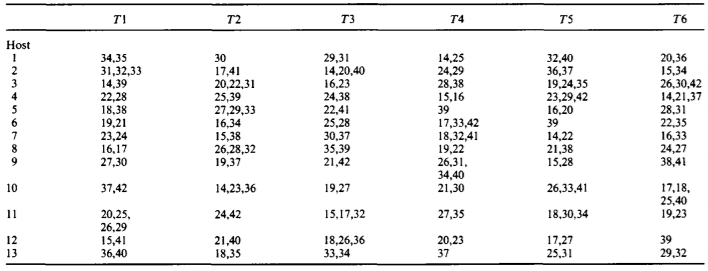
\includegraphics[width=1.0\textwidth]{party3.png}
 \caption{Solución óptima encontrada en ~\cite{Brailsford:1996:OSE:241748.241755}}
\end{figure}
\newpage
Posteriormente, se eliminaron las restricciones adicionales y el programa permite buscar una solución sin esta intervención. Encontró una solución al problema de 42 yates en 27 minutos, y continuó con una solución para el siguiente período de tiempo en otro minuto, de modo que el evento podría haber durado más tiempo sin necesidad de más anfitriones.
\end{itemize}
\end{itemize}

En el paper \textit{Solving Lineal Pseudo-Boolean Constraint Problems with Local Search}~\cite{Walser:1997:SLP:1867406.1867448} se trata el problema con una búsqueda local, el cual es mucho mas eficiente que los otros modelos, pudiendo resolver el problema más rápido. Se introduce la búsqueda local de dominio independiente para satisfacibilidad (\textit{Walksat}), el cual puede generalizarse para manejar sistemas de restricciones lineales pseudo-booleanas. Se introduce de esta búsqueda el algoritmo $\text{W}_{\text{SAT}}$($\mathcal{PB}$) (\textit{WalkSATisfiability}), heurística que sobre problemas de tamaño realista es eficiente para encontrar buenas soluciones aproximadas trabajando con restricciones en el mundo \textbf{de lo factible}, pero su desempeño en estos problemas es a menudo críticamente dependiente de los conceptos incorporados del \textit{Tabu Search} (Como el uso de una lista \textit{Tabu Memory}). Además, para el movimiento del algoritmo, se define un \textit{score}. Este score disminuye a medida que nos quedamos con una nueva solución, llegando a su fin si este \textit{score} llega a 0 (indicador que nos dirá que hemos llegado a la solución óptima). La solución inicial para poder comenzar con el algoritmo se crea con el algoritmo \textit{Greedy} a través de restricciones pseudo-booleanas.

Probando este algoritmo sobre nuestro problema obtenemos lo siguiente:
\begin{figure}[ht]
\centering
 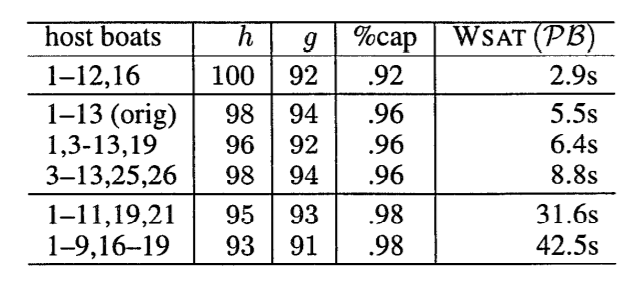
\includegraphics[width=0.6\textwidth]{party4.png}
 \caption{Comparaciones empíricas de las variaciones de PPP}
\end{figure}
\\
Donde las columnas son:

\begin{itemize}
\item \textit{host boats}: Anfitriones seleccionados.
\item \textit{h}: Suma total de las capacidades de holgura del anfitrión $h$.
\item \textit{g}: Suma total del tamaño de las tripulaciones $g$.
\item \textit{\% cap}: Porcentaje de la capacidad total usada como una medida de restricción $g$.
\item $\text{W}_{\text{SAT}}$($\mathcal{PB}$): Promedio de tiempos de ejecución sobre 20 ejecuciones de $\text{W}_{\text{SAT}}$($\mathcal{PB}$)
\end{itemize}

Cada solución con 13 anfitriones es óptima porque las limitaciones de capacidad no se pueden cumplir con 12 anfitriones, ni siquiera por un solo período de tiempo. La solución del problema se puede dividir en dos etapas: 

\begin{itemize}
    \item Selección de los barcos anfitriones.
    \item Asignación de barcos invitados a los anfitriones para todos los períodos de tiempo
\end{itemize}

Por lo que la capacidad disponible de los barcos es un buen indicador de si un barco debe ser anfitrión o invitado, de modo que después de obligar a los barcos a ser anfitriones (por ejemplo, el organizador del club), los anfitriones restantes se seleccionaron disminuyendo la capacidad libre (la capacidad disponible de un barco es su capacidad total menos el tamaño de su tripulación). El tiempo de ejecución de la instancia original descrito en ~\cite{Smith1996} es de 27 minutos, mientras que el tiempo descrito en este paper es de 8 minutos (debido a la limitación computacional de la maquina), tiempo considerablemente mas bajo que los modelos propuestos en ~\cite{Smith1996}. Estas instancias fueron ejecutadas en Oz (un lenguaje de restricciones concurrente) en la maquina SPARCstation 20.

En el paper \textit{Mixed logical-linear programming}~\cite{Hooker1999395} se modela el problema como un MLLP (\textit{Mixed-Logical Lineal Programming}). Se interpreta las variables multivalentes como variables numéricas y hace cumplir las restricciones de forma totalmente diferentes. La complejidad de esto es O(B$^2$T), y la función objetivo sigue siendo encontrar la mínima cantidad de yates anfitriones.
Sin embargo, esto fue probado solo con instancias pequeñas, y con el problema completo aun sigue siendo insoluble.

Cercano al año 2000, el paper \textit{Solving the Progressive Party Problem by Local Search}~\cite{Galinier1999} nos presenta una tercera alternativa para poder resolver nuestro problema, presentando un \textit{approach} de PPP basado en Búsqueda Local. Estos resultados son mejores que los experimentos anteriores y constituyen una alternativa muy eficiente para poder resolver nuestro problema. Formulando el problema como un CSP: tomamos $T$ como el número de periodos, $G$ como el número de botes invitados y $H$ como el número de yates anfitriones. Además, definimos $c(g)$ para denotar el tamaño de una tripulación, donde  $g \in \{ 1,\ldots, G\}$, $C(h)$ la capacidad de un barco anfitrión donde $h \in \{ 1,\ldots H\}$ y $x_{g,t} \in \{ 1,\ldots H\}$ el yate anfitrión visitado por la tripulación g durante el periodo $T$. Como instanciación inicial tenemos H = 13 barcos anfitriones y 29 yates invitados, y la siguiente tabla nos muestra las capacidades de cada barco y el tamaño sus tripulaciones respectivas.

\begin{table}[ht!]
 \centering
    \begin{tabular}{|l|l|l|l|l|}
    \hline
    Capacity C & \#boats & ~ & size c & \#crews \\ \hline
    10         & 2       & ~ & 7      & 1       \\
    9          & 1       & ~ & 6      & 1       \\
    8          & 6       & ~ & 5      & 3       \\
    7          & 1       & ~ & 4      & 8       \\
    6          & 1       & ~ & 3      & 2       \\
    4          & 1       & ~ & 2      & 14      \\ \hline
    ~          & 13      & ~ & ~      & 29      \\ \hline
    \end{tabular}
        \caption{Capacidad de los botes y el tamaño de las tripulaciones}
\label{table:capacidad}
\end{table}

Debemos tener en cuenta sin embargo, que un límite superior obvio para T es 10. De hecho, hay un equipo de invitados de tamaño 7 y sólo 10 \textit{hosts} tienen una capacidad mayor o igual a 7. Por lo tanto, sólo 10 \textit{hosts} pueden ser asignados a esta tripulación de invitados con el fin de respetar la limitación de capacidad. Por otra parte, esta tripulación de invitados debe visitar un anfitrión diferente en cada período de tiempo. Por lo tanto, el número de períodos de tiempo no puede excederse de 10. Las restricciones definidas son: 

\begin{itemize}
    \item El primer tipo de restricción impone que cada tripulación se mueva a un anfitrión diferente en cada período de tiempo, la cual se denominan DIFF($g$),
    \item El segundo tipo de restricción impone que dos tripulaciones se reúnan a lo sumo una vez: para cada par de tripulaciones invitadas, el número de periodos de tiempo en que se reúnen estas dos tripulaciones es 0 o 1. Se denomina como ONCE(\{$g1,g2$\}).
    \item El tercer tipo de restricción impone que se respete la capacidad de los barcos anfitriones. Se denomina como CAPA ($h,t$). 
\end{itemize}

las cuales son similares al modelo CSP de ~\cite{Smith1996}. 
Como se ha expuesto anteriormente, una configuración es una asignación completa de los números en $D = {1,\ldots ,H = 13}$ a las variables de $X = {x_{gt}, 1 \leq g \leq G, 1 \leq t \leq T}$. 
 La configuración es una tabla $G \times T (G = 29 \text{ y } T = 6,7,8,9 \text{ o }10)$ cuyos elementos son números enteros de $\{1\ldots 13\}$. El espacio de búsqueda es el conjunto de todas estas asignaciones. Además, se plantea una función de costos, la cual se define como el número de restricciones violadas, asociando a cada restricción $C$ una penalidad $f_C (s)$ que toma 1 o 0 según que la restricción sea violada o no. De hecho, esta función no puede distinguir una restricción "fuertemente violada" de una "débilmente" violada. En el PPP, las restricciones son más complejas, por lo que se proponen una función de \textit{penalty} para las restricciones ~\cite{Galinier1999}. Luego, la función de costo (evaluación) nos queda como la suma de la multiplicación entre unos pesos $p$ (varían dependiendo de cada función) y las funciones de \textit{penalty} $f_{C}$. 

Cabe destacar que a diferencia de los demas modelos que trabajaban en el mundo de lo factible, estos algoritmos trabajan en el mundo \textbf{de lo infactible}.
Definimos entonces dos tipos de movimientos:
\begin{itemize}
    \item \textit{OneMove}: \\
    Un movimiento del tipo OneMove consiste simplemente en cambiar un barco anfitrión a una tripulación dada por un período dado.
    
    \item \textit{Swap}: \\
    Un movimiento \textit{swap} consiste en invertir los barcos anfitriones asignados a dos tripulacion $g_1$ y $g_2$ durante el mismo periodo de tiempo $t$. 
\end{itemize}

Teniendo esto, se definen 2 principales tipos de meta-heurísticas: \textit{Metropolis algorithm} y \textit{Tabu Search algorithm}. 

\begin{itemize}
 \item \textbf{\textit{Metropolis algorithm}}: \\
 El algoritmo Metrópolis es una versión simplificada de \textit{Simulated Annealing} que utiliza un valor constante para su parámetro de temperatura. El algoritmo comienza con una configuración inicial en el espacio de búsqueda y luego realiza una serie de iteraciones. En cada iteración, se elige aleatoriamente un solo vecino (o equivalentemente un solo movimiento) de la configuración actual y luego se realiza un criterio probabilístico para decidir si este vecino es aceptado o no. El principio del algoritmo Metrópolis es aceptar cualquier movimiento que no aumente la función de coste, y aceptar, de manera controlada, movimientos de deterioro. Así se asegura de que el algoritmo no quede atrapado en un óptima local.
 
El método tiene un parámetro $\theta$ llamado temperatura: cuanto más alto es el valor de la temperatura, se aceptan las degradaciones más fáciles (una temperatura cero corresponde a un descenso ya que todos los movimientos de deterioro son rechazados mientras que una temperatura infinita es realizar muchos cambios aleatorios en el espacio de búsqueda, ya que todos los movimientos son aceptados).

\item \textbf{\textit{Tabu search}}: \\
El algoritmo búsqueda de tabú comienza con una configuración inicial en el espacio de búsqueda y luego procede iterativamente a visitar una serie de configuraciones localmente mejores siguiendo el vecindario. En cada iteración, se aplica un mejor movimiento a la configuración actual , incluso si la solución no mejora la configuración actual en términos del valor de la función de coste. 

Este proceso iterativo puede sufrir ciclismo y quedar atrapado en un óptimo local. Para evitar este problema, TS introduce la noción de listas Tabú. Una lista tabú es una lista especial de corto plazo que mantiene un historial, compuesta de soluciones previamente encontradas. Una estrategia de TS simple basada en esta lista de corto plazo consiste en evitar que las soluciones guardadas sean reconsideradas para próximas $k$ iteraciones. \end{itemize}

En la siguiente tabla se presentan los resultados computacionales de diferentes modelos en distintos periodos de tiempo:

\begin{table}[ht!]
\centering
    \begin{tabular}{|c|l|c|c|c|c|}
    \hline
    problem & ~ & ILP  & CP1     & CP2        & LS     \\ \hline
    P6      & ~ & fail & 27 min. & a few sec. & $<$ 1 s. \\
    P7      & ~ & fail & 28 min. & a few sec. & $<$ 1 s. \\
    P8      & ~ & fail & fail    & a few sec. & 1 s.   \\
    P9      & ~ & fail & fail    & hours      & 4 s.   \\
    P10     & ~ & fail & fail    & fail       & fail   \\ \hline
    \end{tabular}
    \caption{Resultados de distintos algoritmos para PPP}
\label{table:kysymys}
\end{table}

Donde las columnas significan:
\begin{itemize}
    \item \textit{problem}: Distintos periodos $P_i$ del problema.
    \item \text{ILP}: Modelado de PPP con Algoritmo de Programación Lineal Entera propuesto en ~\cite{Smith1996}.
    \item{CP1}: Modelado de PPP como un CSP, relajando ciertas restricciones, también propuesto en ~\cite{Smith1996}.
    \item{CP2}: Una nueva estrategia llamada \textit{Partial Search Method} es implementada y probada en el \textit{solver} CHIP ~\cite{CHIP1997}. 
    \item Resultados con las búsquedas locales previamente definidas, corriendo estos experimentos en C++ y ejecutada en la maquina Sun ULTRA 1.
\end{itemize}

Cada experimento se corrió 20 veces, demostrando claramente que las búsquedas locales tienen un tiempo promedio mucho mas bajo que el resto. Cabe destacar que en el periodo 10 todos los métodos parecen fallan en entregar un resultado. Observando el periodo 9, nos damos cuenta de que la búsqueda local cobra una fuerte ventaja de tiempo frente a los otros algoritmos, por lo que es un caso muy interesante a considerar y analizar. Analizando sus costos observamos lo siguiente:

\begin{table}[!ht]
\centering
    \begin{tabular}{|c|c|c|c|c|c|c|c|}
    \hline
    ~     & [0..5[ & [5..10[ & [10..15[ & [15..20[ & [20..25[ & [25..30[ & [30..35[ \\ \hline
    $\psi_1(\%)$  & 1.7    & 1.4     & 15.6     & 37.3     & 42.3     & 42.8     & 52.0    \\
    $\psi_2(\%)$ & 10.3   & 41.1    & 51.2     & 60.6     & 67.1     & 67.9     & 69.5    \\ \hline
    \end{tabular}
    \caption{Porcentaje de costos para los movimientos \textit{OneMove} y \textit{Swap}}
\label{table:porcentajes}
\end{table}

Donde cada columna nos indica el porcentaje de las soluciones que tuvieron un costo dentro de los rangos correspondientes. Por ejemplo, en la primera segunda columna de la tabla, observamos que en el movimiento 2 el $1.7\%$ de los resultados obtenidos obtuvieron un costo entre 0 y 5, mientras que el movimiento dos obtuvo un $10.3\%$. Esto nos sirve para comparar ambos movimientos, concluyendo que el segundo movimiento fue mucho mejor y eficiente que que el primer movimiento.

Ya en el 2009, el paper \textit{Progress on the Progressive Party Problem} ~\cite{Simonis2009} nos entrega otro \textit{approach} de la solución usando \textit{finite domain constraints}, donde las variables tienen dominios finitos y se pueden eliminar
valores de los dominios durante la ejecución del problema. Aqui se busca entontrar soluciones para distintos periodos de tiempos, yates anfitriones o yates invitados. El primer modelo planteado para las restricciones es el siguiente:

\begin{itemize}
    \item \textit{alldifferent}: Este tipo de restricciones nos señala que se instancian valores diferentes para un conjunto de variables. Se aplica a la restricción de que una tripulación invitada no podrá visitar un yate anfitrión más de una vez.
    \item \textit{bin-packing}: Este tipo de restricciones agrupar cosas eficientemente dentro de un recipiente (\textit{bin}). Se aplica a la restricción de que la capacidad de los yates anfitriones no se puede exceder.
    \item \textit{Equality reified}: Este tipo de restricciones asocia valores \textit{de verdad} a una restricción. Se aplica a la restricción de que las tripulaciones invitadas no podrán toparse más de una vez.
\end{itemize}
Sin embargo, hubieron problemas con este modelo, puesto que no existía mucha propagación de restricciones y no había mucha interacción entre los diferentes periodos de tiempo. Por esto, se planteo un segundo modelo donde se descompone el problema por periodos, y resolviendo cada periodo por separado. Así, al resolver la primera instancia, se agregarían restricciones en base a las asignaciones para el segundo periodo, realizando esto para los siguientes $k$ periodos En el segundo modelo se consideran las siguientes variantes: se propone que la próxima variable a asignar debe ser la que es más probable que falle (\textit{first\_fail}), puesto que el mayor costo del algoritmo era realizar un \textit{backtracking} demasiado profundo. Por cada periodo además, se usó una estrategia de búsqueda parcial, la cual limita el numero de \textit{backtraking}, reduciendo el costo de buscar por todo el árbol (búsqueda conocida como \textit{credit search}). Finalmente se agrega aleatoriedad al momento de asignar valores para que haya un desorden en la elección de valores, para no quedar atrapados en una rama del árbol y poder así explorar otras soluciones.

Realizando estos cambios, se noto una mejora ejecución y no se perdió propagación.





\section{Modelo Matemático}
Se presenta la primera formulación del problema \textit{Progressive Party Problem }, descrito de la siguiente manera:

\begin{itemize}
    \item Variables:
    \begin{itemize}
        \item $h_i$: 1 si el yate $i$ es un yate anfitrión
        \item $x_{ikt}$: 1 si el yate $k$ es un invitado del yate $i$ en el periodo $t$. (El dueño del yate organizador del club esta restringido a ser anfitrión en todos los modelos).
        \item $m_{klt}$: 1 si la tripulación $k$ y la tripulación $l$ se encuentran en el periodo $t$.
    \end{itemize}
    \item Función objetivo:
    \begin{itemize}
        \item Minimizar $\displaystyle \sum_{i} h_i$
    \end{itemize}
    \item Restricciones:
    \begin{align}
        \displaystyle x_{ikt} - h_i &\leq 0           & \text{para todo } i,k,t;i\neq k  \\ 
        \displaystyle \sum_{k,k\neq i} c_k x_{ikt} & \leq g_i & \text{para todo } i,t \\
        & & \text{ donde } g_i  \text{: max} \{K_i - c_i,0 \} \\
        \displaystyle \sum_{i,i\neq k} x_{ikt} + h_k &= 1            & \text{para todo }k,t \\
        \displaystyle \sum_{t} x_{ikt} &\leq 1            & \text{para todo } i,k;i \leq k \\
        \displaystyle m_{klt} &\geq x_{ikt} + x_{ilt} -1           & \text{para todo } k,l,t; k<l \\
        \displaystyle \sum_{t} m_{klt} &\leq 1 & \text{para todo } k,l,t; k<l
    \end{align}
    Sobre las restricciones:
    \begin{itemize}
        \item (1) Un bote solo puede ser visitado si es un yate anfitrión.
        \item (2) La capacidad de un yate anfitrión no puede ser excedida. Además, $c_i$ es el tamaño de la tripulación del bote $i$ y $K_i$ es la capacidad total del yate.
        \item (3) Cada tripulación debe tener al menos un yate anfitrión.
        \item (4) Una tripulación no puede visitar un yate anfitrión mas de una vez. 
        \item (5) y (6): Como el barco anfitrión i es irrelevante, la siguiente formulación es más apropiada que en ~\cite{Walser:1997:SLP:1867406.1867448}. Se define la variable binarias $m_{klt}$ en lugar de $y_{iklt}$ que toma el valor 1 si las tripulaciones k y l se reúnen en el instante t. Si no se reúnen entonces, dejamos $m_{klt}$ sin restricciones.
    \end{itemize}
\end{itemize}
Nuestro espacio de busqueda nos quedaria de la siguiente forma:
\begin{itemize}
    \item $h_i$: todo su espacio seria de $2^{13}$, puesto que son 13 barcos anfitriones, y cada uni puede tomar el valor de 0 o 1.
    \item $x_{ikt}$: todo el espacio a abarcar por esta variable es de $2^{42\cdot39\cdot}$, puesto que son 42 yates, 39 tripulaciones (las tripulaciones virtuales se setean como 0, por lo que no cuentan) y los periodos son 6 (3 horas).
    \item $m_{klt}$: todos los valores posibles que puede tomar esta variable son $2^{42\cdot42\cdot6}$, puesto que las tripulaciones \textit{host} si cuentan, aunque no se mueven de sus barcos. Siendo asi, 42 son las tripulaciones y 6 los periodos.
\end{itemize}
Teniendo esto, el espacio de busqueda queda definido como:
\begin{align*}
    EB = 2^{13} \cdot 2^{42\cdot39\cdot6} \cdot 2^{42\cdot42\cdot6}
\end{align*}

Alternativamente se propone un segundo modelo como CSP, el cual es un poco más compacto. Supongamos que tenemos $G$ barcos invitados, $H$ yates \textit{host} y $T$ periodos:
\begin{itemize}
    \item Variable:
    \begin{itemize}
        \item $h_{it}$: Yate anfitrión que el yate invitado $i$ visito en el periodo $t$.
        \item Dominio $h_{it}$: $\{1,\ldots H \}$, con un total de $GT$ variables.
    \end{itemize}
    \item Restricciones:
    \begin{itemize}
        \item La restricción de que cada barco invitado debe tener siempre un anfitrión y que en cualquier período de tiempo un barco invitado sólo puede ser asignado a un \textit{host} son automáticamente satisfechas por cualquier solución del CSP, donde exactamente se asigna un anfitrión a cada barco invitado en cada período de tiempo.
        \item La restricción de que ningún barco invitado puede visitar un barco anfitrión más de una vez en el modelo CSP se expresa como:
        \begin{align*}
            &h_{i1},h_{i2},h_{i3},\ldots h_{iT} \text{ sean todos distintos para todo } i\neq k \\
            &h_{i1} \neq h_{i2}, \ldots 
        \end{align*}
        Donde para cada $i$, esto no es mas que una restricción de tipo \textit{Solve} para el problema, quedando $\displaystyle\frac{T(T-1)}{2}$  restricciones binarias desiguales.
        \item Las restricciones de capacidad son tratadas como en LP:
        \begin{align*}
            v_{ijt} = 1 \text{ si y solo si } h_{it} = j, \text{ para todo } i,j,t.
        \end{align*}
        Donde la relacion entre $v_{ijt}$ y $h_{it}$ es de GHT variables booleanas. Finalmente la restricción de capacidad nos queda como:
        \begin{align*}
            \sum_{i} c_{i}v_{ijt} \leq C_j, \text{ para todo } j,t.
        \end{align*}
        
        Donde $c_i$ es el tamaño de la tripulación de invitado barco $i$ y $C_j$ es la capacidad de reserva del barco anfitrión $j$, después de acomodar a su propia tripulación.
        
        \item La restricción de que ningún par de tripulaciones pueda encontrarse dos veces también requiere de una nueva variable binaria:
        \begin{align*}
            \text{si } h_{kt} = h_{lt} \text{ entonces } m_{klt} = 1, \text{ para todo } k,l,t; k<l.
        \end{align*}
        Por lo tanto la restricción de encuentro queda como:
        \begin{align*}
            \sum_{t} m_{klt} \leq 1 ,\text{ para todo } k,l;k<l
        \end{align*}
    \end{itemize}
\end{itemize}


\section{Conclusiones}
La planificación de tiempos es un amplio campo a optimizar y posee grande aplicaciones en la vida real, por lo que es clave poder desarrollar técnicas que permitan entregar una correcta gestión de estos elementos. A pesar de que el \textit{Progressive Party Problem} estudiado es una versión simplificada del problema que debe ser aplicado en la vida real, fue un
problema de vital importancia en el desarrollo del área pues permitió sentar las bases de los avances que se han logrado en los problemas derivados. El problema puede ser atacado con algoritmos que tienen distintos enfoques y trabajan
de maneras completamente distinta, pero no aseguran que el problema pueda resolverse de forma rápida y eficiente.

Por otra parte se analizaron ciertas variantes del problema, las cuales ayudaron de manera significativa al desarrollo y mejora de los algoritmos posteriormente presentados, tales como la cantidad de yates anfitriones y yates invitados, instancia usada en varios planteamentos posteriores.

En el paper \textit{The progressive party problem: Integer linear programming and constraint programming compared} ~\cite{Smith1996} se analizaron dos modelos para el análisis y resolución del PPP: Programación Lineal Entera y Programación de restricciones. Sin embargo, para el primer caso fue imposible resolver el modelo real en su totalidad (incluso relajando el problema), y para el caso de CSP fue necesaria una relajación del problema para poder abordarlo y poder entregar una solución en un tiempo prudente. A pesar de ser razonable en cierta parte la gran demora de tiempo que estos algoritmos presentan, debido a las limitaciones computacionales de ese año, se ha podido trabajar y mejorar el modelo de PPP, entregando resultados sorprendentes en comparación a estos dos modelos.

En el paper \textit{Solving Lineal Pseudo-Boolean Constraint Problems with Local Search}~\cite{Walser:1997:SLP:1867406.1867448} se resuelve el problema usando una búsqueda local para la búsqueda de soluciones, e introduciendo el algoritmo $\text{W}_{\text{SAT}}$($\mathcal{PB}$) , heurística que sobre problemas de tamaño realista es eficiente para encontrar buenas soluciones aproximadas trabajando con restricciones en el mundo de lo factible, introduciendo recursos para que el algoritmo funcione correctamente (como el movimiento, la creación de una solución inicial (\textit{Greedy}) o la lista Tabú). Probando este algoritmo sobre nuestro problema nos damos cuenta que los tiempos bajan de forma considerable en comparación a lo planteado en ~\cite{Smith1996}, además de que a pesar de ser una búsqueda local y no global, encuentra soluciones bastante eficientes. 

Posteriormente en el paper \textit{Solving the Progressive Party Problem by Local Search}~\cite{Galinier1999}se nos presenta una tercera alternativa para poder resolver nuestro problema, presentando otro \textit{approach} de PPP basado en búsqueda local. Se resuelve el problema usando dos meta-heurísticas, las cuales son \textit{Metropolis algorithm} y \textit{Tabu Search algorithm}. Además, se definen dos movimientos los cuales son \textit{OneMove} y \textit{Swap}, además de una función de evaluacion en base a costos y \textit{penalty}'s (definidos como pesos) y a través de los experimentos se decide que movimiento es mejor. Claramente comparando estos métodos con los otros modelos estudiados podemos apreciar la alta reducción de tiempo que presentan las búsquedas locales frente a los otros métodos descritos en ~\cite{Smith1996}, por lo que las búsquedas locales son ideales para resolver estos problemas.

Finalmente en el paper \textit{Progress on the Progressive Party Problem} ~\cite{Simonis2009} se nos entrega otro \textit{approach} de la solución usando \textit{finite domain constraints}, donde las variables tienen dominios finitos y se pueden eliminar valores de los dominios durante la ejecución del problema. Haciendo distintos cambios a las restricciones  y aplicando nuevos elementos (como \textit{credit search}, aleatoriedad, descomponer el problema en periodos, etc) nos damos cuenta de que se puede seguir optimizando el modelo, logrando así una solución más rápida al problema.


Por lo visto en los experimentos, se puede concluir que conviene buscar una solución local mas que una global (\textit{puntualizar y no en generalizar}), concepto que cada vez se hace mas recurrente en la Inteligencia Artificial. Seria importante analizar a cabalidad más algoritmos de búsqueda local, de forma de definir mejores movimientos que puedan afectar de forma positiva el tiempo de ejecución del problema.

Es importante destacar, para concluir este informe, que aun quedan muchas áreas que investigar y muchos métodos que desarrollar y combinar para poder desarrollar nuestro problema de forma más eficiente y rápida.  



\bibliographystyle{plain}
\bibliography{Referencias}

\end{document} 